\documentclass[12pt, a4paper]{article}
\usepackage[utf8]{inputenc}
\usepackage{amsmath}
\usepackage{amsfonts}
\usepackage{amsthm}
\usepackage{array}
\usepackage{graphicx}
\usepackage{parskip}
\usepackage[pdfencoding=auto]{hyperref}
\usepackage{fancyhdr}
\usepackage{lastpage}
\usepackage{tikz}
\usepackage{float}
\usepackage{listings}
\usepackage{color}
\usepackage{caption}
\usepackage{authblk}
\usepackage[acronym]{glossaries}
\usepackage[nottoc]{tocbibind}
\usepackage[cache=false]{minted}
\usemintedstyle{default}
\newminted{haskell}{frame=lines,framerule=2pt}
\newminted{R}{frame=lines,framerule=2pt}
\graphicspath{{./images/}}

\tikzstyle{bag} = [align=center]

\title{%
      Homework 2\\
      Degree Distribution Analysis\\
}
\author{Juan Pablo Royo Sales \& Francesc Roy Campderrós}
\affil{Universitat Politècnica de Catalunya}
\date\today

\pagestyle{fancy}
\fancyhf{}
\fancyhead[C]{}
\fancyhead[R]{UPC MIRI}
\fancyhead[L]{CSN - Homework 2}
\fancyfoot[L,C]{}
\fancyfoot[R]{Page \thepage{} of \pageref{LastPage}}
\setlength{\headheight}{15pt}
\renewcommand{\headrulewidth}{0.4pt}
\renewcommand{\footrulewidth}{0.4pt}

\newacronym{indegree}{Incomming Degree}{Incomming Degree Language Set}
\newacronym{dispp}{Displaced Poisson}{Displaced Poisson Model}
\newacronym{dispg}{Displaced Geometric}{Displaced Geometric Model}
\newacronym{zeta2}{Zeta-Gamma-2}{Zeta Model with fixed Gamma with value 2}
\newacronym{zeta}{Zeta}{Zeta Model}
\newacronym{zetar}{Right-Truncated Zeta}{Right-Truncated Zeta Model}
\newacronym{aic}{Akaike}{Akaike Information Criterion}
\newacronym{alt}{Altmann}{Altmann Model}

\begin{document}

\maketitle

\tableofcontents

\section{Introduction}
In this homework we have analyzed \acrfull{indegree}~\ref{apx:src:1} which contains the distribution over different natural languages for the incomming connection words frequency.

The goal of this work is to analyzed according to what have been discussing in class, what is the best model that fits (or explain), this distribution over the whole set of languages, taking into consideration
only \textbf{five} different models: \acrfull{dispp}, \acrfull{dispg}, \acrfull{zeta2}, \acrfull{zeta} and \acrfull{zetar}

Additionally we are going to compare these results using \acrfull{aic} in order to determine what model fits best for each language. 

At the end of the work the we are going to run the distribution against \acrfull{alt}, that has been pointed out during the lectures to fit better. 

This analysis work is going to be done in the following way:

\begin{itemize}
    \item \textbf{Results} section: We are going to show the results obtained for each language according to the previous statements.
    \item \textbf{Discussion and Methods} section: In this section we are going to conclude and give some explanaition based on the results.
    \item \textbf{Conclusions} section: Finally we are going to give our opinion about the results obtained and what we have learnt.
\end{itemize}

\section{Results}
Lets divide the results for each language, but first lets see the Summary of the data that we are analysing.

\subsection{Distributions}

\begin{table}[H]
    \centering
    \begin{tabular}{p{2cm} p{2cm} p{2cm} p{3cm} p{3cm}}
    Language & N & Maximum degree & M/N & N/M\\
     \hline
     Arabic    & 21065 & 2249 & 3.35100878234037 & 0.298417600475995\\
     Basque    & 11868 & 576  & 2.18031681833502 & 0.458648941103725\\
     Catalan   & 35524 & 5522 & 5.74527080283752 & 0.174056199318945\\
     Chinese   & 35563 & 7645 & 5.20240137221269 & 0.192218925156611\\
     Czech     & 66014 & 4727 & 3.97215742115309 & 0.25175235872442 \\
     English   & 29172 & 4547 & 6.8572946661182  & 0.14583010482851 \\
     Greek     & 12704 & 1081 & 3.52392947103275 & 0.283774124374553\\
     Hungarian & 34600 & 6540 & 3.09763005780347 & 0.322827445931068\\
     Italian   & 13433 & 2678 & 4.23055162659123 & 0.236375794048813\\
     Turkish   & 20403 & 6704 & 2.31269911287556 & 0.432395201966685
    \end{tabular}
   \caption{Language List - Paramters}
   \label{table:1}
\end{table}

\subsection{Fitting Model Results}
Lets remind the model classification in the Appendix section~\ref{apx:table:model:clasification}

\begin{table}[H]
\centering
    \begin{tabular}{l c c c c}
             & 1 & 2 & 4 & 5\\
    Language & $\lambda$ & $q$ & $\gamma$ & $k_{max}$\\
     \hline
     Arabic    & 3.216673 & 0.2984176 & 2.104113 & 24065 \\
     Basque    & 1.830868 & 0.4586489 & 2.358005 & 14868 \\
     Catalan   & 5.726551 & 0.1740562 & 1.922218 & 38524 \\
     Chinese   & 5.172914 & 0.1922189 & 1.885594 & 38563 \\
     Czech     & 3.891029 & 0.2517524 & 2.050873 & 69014 \\
     English   & 6.850030 & 0.1458301 & 1.799843 & 32172 \\
     Greek     & 3.407164 & 0.2837741 & 2.131930 & 15704 \\
     Hungarian & 2.932666 & 0.3228275 & 2.335141 & 37600 \\
     Italian   & 4.164842 & 0.2363758 & 2.108419 & 16433 \\
     Turkish   & 1.999577 & 0.4323952 & 2.543344 & 23403 
    \end{tabular}
   \caption{Model Fitting by Language}
   \label{table:3}
\end{table}

\subsection{AIC Results}
\begin{table}[H]
\centering
    \begin{tabular}{l c c c c c}
    Language & AIC 1 & AIC 2 & AIC 3 & AIC 4 & AIC 5\\
     \hline
     Arabic    & 240318.35 & 24186.041 &  172.3717 & \textbf{0.0000000} & 1.643912\\          
     Basque    &  50164.36 &  8363.878 &  845.1732 & \textbf{0.0000000} & 1.973784\\          
     Catalan   & 913866.77 & 61868.421 &  212.5898 & 0.6420711 & \textbf{0.000000}\\          
     Chinese   & 618335.67 & 48666.087 &  491.2543 & 1.9569369 & \textbf{0.000000}\\          
     Czech     & 940668.86 & 91090.542 &  138.4353 & \textbf{0.0000000} & 1.354231\\          
     English   & 739544.11 & 45704.816 & 1432.2985 & 7.6821378 & \textbf{0.000000}\\          
     Greek     & 157133.81 & 17130.408 &  160.6789 & \textbf{0.0000000} & 1.740389\\          
     Hungarian & 468252.20 & 53469.625 & 2220.2829 & \textbf{0.0000000} & 1.971684\\          
     Italian   & 245803.03 & 22877.409 &  117.8825 & \textbf{0.0000000} & 1.668910\\          
     Turkish   & 193345.03 & 24615.351 & 2740.4657 & \textbf{0.0000000} & 1.996789 
    \end{tabular}
   \caption{AIC Results}
   \label{table:4}
\end{table}

\subsection{Altmann Results}
\begin{table}[H]
    \centering
        \begin{tabular}{l c c}
        Language & $\gamma$ & $\delta$ \\
         \hline
         Arabic    & 2.086211 & 0.0014726478 \\
         Basque    & 2.346528 & 0.0017016417 \\
         Catalan   & 1.907315 & 0.0008281837 \\
         Chinese   & 1.834734 & 0.0028665707 \\
         Czech     & 2.035468 & 0.0010169897 \\
         English   & 1.740599 & 0.0025428652 \\
         Greek     & 2.131722 & 0.0000010000 \\
         Hungarian & 2.335120 & 0.0000010000 \\
         Italian   & 2.108182 & 0.0000010000 \\
         Turkish   & 2.543335 & 0.0000010000 
        \end{tabular}
       \caption{Altmann Results}
       \label{table:5}
    \end{table}

\section{Discussion and Methods}
\subsection{Considerations}
It is known that all the likelihood functions has been provided and the only thing that need to be adjust it to negate them.
On the other hand there it is important to point out that the \textbf{lower} and \textbf{upper} bound parameters needs to be adjust for each case.
The idea here is to explain those consideration that we have taken into account for each Model.

\subsubsection{Zeta Model}
In this case as we can see $\gamma = 1.0000001$ as lower bound and $\gamma = 2$ as an started point
\begin{listing}[H]
    \inputminted[firstline=59, lastline=67, breaklines]{R}{./Solution.R}
    \caption{Extracted from source Solution.R}
    \label{apx:src:2}
\end{listing}  

\subsubsection{Zeta Truncated}
One of the important setup on this model was start value of $k_{max}$. Since it is known that $k \gg N$ we cannot put as a started value of $k_{max} = N$
because on some cases, particularly in \textbf{English}, this cannot be optimized. Therefore we have chosen $k_{max} = N + 3000$ as a started value which is $\gg N$. 
\begin{listing}[H]
    \inputminted[firstline=70, lastline=83, breaklines]{R}{./Solution.R}
    \caption{Extracted from source Solution.R}
    \label{apx:src:3}
\end{listing}  

\subsubsection{Displaced Poisson and Geometric}
On those cases we have done the regular setup but taking into consideration that we are calculating $C$ value from the sample.
\begin{listing}[H]
    \inputminted[firstline=11, lastline=19, breaklines]{R}{./Solution.R}
    \caption{Extracted from source Solution.R}
    \label{apx:src:4}
\end{listing}  
\begin{listing}[H]
    \inputminted[firstline=86, lastline=95, breaklines]{R}{./Solution.R}
    \caption{Extracted from source Solution.R}
    \label{apx:src:5}
\end{listing}  


\subsection{General Analysis}
As we can see in the table~\ref{table:4} the best models are between \acrshort{zeta} and \acrshort{zetar} because 
are the ones in which the $\Delta = AIC - AIC_{best}$ is the smallest. As long as the $AIC$ value approximates to the
best possible value that difference approximates to $0$, indicating that the prediction is fitting the model better for all languages
in general.

If we have to pick only \textbf{one} model which fits better for all languages, according to the \acrshort{aic} results this should be \acrshort{zeta}. This is 
pretty obvious since in almost all languages $\Delta = 0$. For the rest of the languages which are not $0$, like \textbf{Catalan, Chinese and English}, it is 
still an small difference and it can be explain that it is also a good model.

In these cases as we can see in the distribution table~\ref{table:1} $M/N$ the average degree frequency is higher for those $3$ languages. In those cases since it is 
clear that we have more degrees frequencies in few terms the distribution is not straightforward enough to be fitted by a \acrshort{zeta} model and we might be needing more
parameters to fit better the model. And that the case of \acrshort{zetar}.

Taking into consideration that we are analyzing a \acrshort{indegree} $\{w | (u,w) \in E\}$, this means all the words that have edges from some other words connecting to this.
Although we cannot give an intuitive explanation for \textit{Chinese}, for the case of the \textit{Catalan and English} it is clear that those words are connectors and/or 
prepositions in the language like \textit{in, at, of, etc} for \textbf{English} or \textit{a, amb, des, dalt, etc} for \textbf{Catalan}. In that case it is straightforward to 
see for someone who speak those languages that there are a lot of this kinds of words with high incoming degree, turning the \textbf{power law} like distribution, not so clear 
on the distribution tail. This would explain that we need extra parameters for fitting the model best when the degree is higher.

On the other hand as well as \acrshort{zeta} is the best function to fit the model, we can appreciate that \acrshort{dispp} is the worst for fitting them. This could be explain
because \textit{Poisson} distribution approximates well when $p$ probability is low and $m$ the number of elements is big. As we are working with an reduce number of terms of the languages,
in this case \acrshort{indegree}, the distribution is not fitting accordingly. 

\subsection{Altmann Model}
One of the topic proposal in the homework was to use an \acrshort{alt} function which it is known that approximates better to the model.
In order to do that we need first to derive \textbf{Log Likelihood} function.

\begin{subequations}
    \begin{align}
        \L &= \sum_{i=o}^N \log{[ck_i^{-\gamma} e^{-\delta k_i}]}\\
           &= \sum_{i=o}^N \log(c) + \log{k_i^{-\gamma}} + (-\delta k_i) log(e)\\
           &= \sum_{i=o}^N \log(c) + -\gamma \log(k_i) + (-\delta k_i) \\
           &= N\log(c) -\gamma M' -\delta M  \\
    \end{align}
    \end{subequations}

As we can see in the table of results~\ref{table:5} $\gamma$ parameters fits well regarding \acrshort{zeta} which is the one
that explain better the model.

\section{Conclusions}
In conclusion we can say that we have learnt how to pick a good Model for fitting a real network with the tools provided. 
Although that and taking into consideration that we have \acrshort{aic} for measuring the accuracy of the model, we can notice the big difference
between the different models such as \acrshort{dispp} and \acrshort{zeta} for example.
This leads to think to the fact that without proper measuring tools like \acrshort{aic} it is really difficult to determine what is the best model. 

On the other hand, the difference is quite strong which indicates that real networks are difficult to predict because of its particular behavior, as we have
explained in the previous section for example the case of \textbf{English} or \textbf{Catalan} where some specific details in the language
can lead to a not straightforward \textbf{Power Law like} distribution.

To sum up we think it has been a great exercise to put in practice the theoretical concepts we have seen in class, but with a real case.

\printglossary[type=\acronymtype]

\appendix\label{apx:org}
\section{Source Code Considerations}
If you want to run \mintinline{bash}{./Solution.R} script to compare the results in this technical report with the sample, you need to take into consideration the following:

\begin{itemize}
    \item \textbf{stats4} package is required to be installed in your \textbf{R} Studio
    \item \textbf{VGAM} package is required to be installed in your \textbf{R} Studio
    \item Unzip \mintinline{bash}{./in-degree_sequences.tar.gz} in the same Root folder of the script. The script is looking for \mintinline{bash}{./data/LANG_in_degree_sequence.txt} 
    files to be placed in a folder in the same place that the script is running. Sometimes you need to setup as a working directory in your \textbf{R} Studio the folder of the script.
    \item Place \mintinline{bash}{./list_in.txt} in the same root folder of the script. Same as previous item.
\end{itemize}

\section{Listing with Languages Files}
\begin{listing}[H]
    \inputminted[breaklines]{text}{./list_in.txt}
    \caption{Extracted from source list\_in.txt}
    \label{apx:src:1}
\end{listing}  

\section{Model Classification}\label{apx:table:model:clasification}
\begin{table}[H]
    \centering
        \begin{tabular}{c c}
        Model & Function \\
         \hline
         1 & Displaced Poisson \\
         2 & Displaced geometric \\
         3 & Zeta with $\gamma = 2$\\
         4 & Zeta \\
         5 & Right-truncated zeta\\
        \end{tabular}
       \caption{Model Classification}
       \label{table:2}
    \end{table}

\section{Plotting}\label{apx:section:plotting}
\begin{minipage}[t]{\linewidth}
    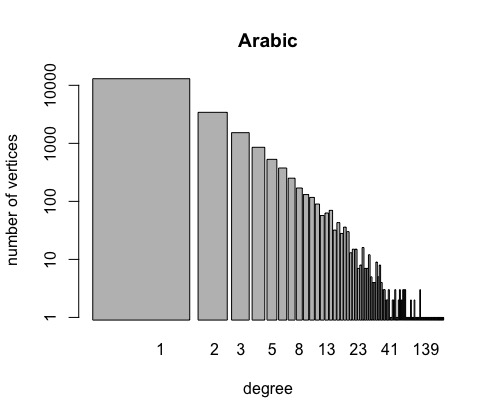
\includegraphics[width=\textwidth]{arabic}
    \captionsetup{type=figure}
    \captionof{figure}{Arabic In Degree}
    \label{fig:arabic}
  \end{minipage}

  \begin{minipage}[t]{\linewidth}
    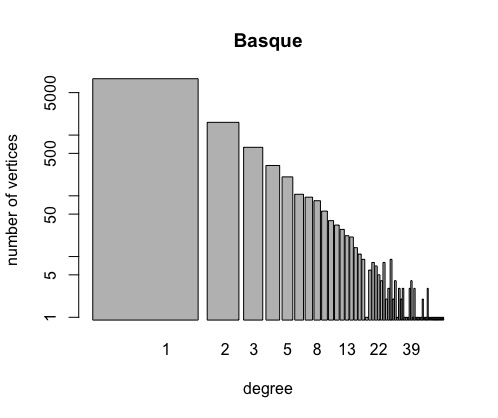
\includegraphics[width=\textwidth]{basque}
    \captionsetup{type=figure}
    \captionof{figure}{Basque In Degree}
    \label{fig:basque}
  \end{minipage}

  \begin{minipage}[t]{\linewidth}
    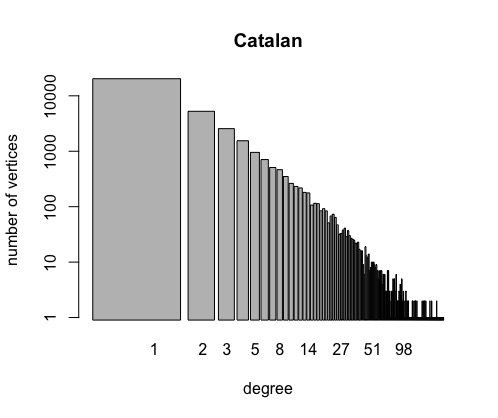
\includegraphics[width=\textwidth]{catalan}
    \captionsetup{type=figure}
    \captionof{figure}{Catalan In Degree}
    \label{fig:catalan}
  \end{minipage}

  \begin{minipage}[t]{\linewidth}
    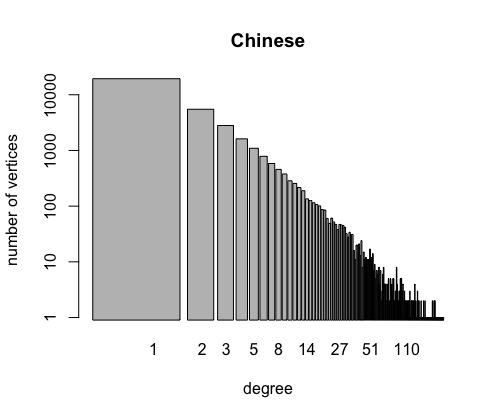
\includegraphics[width=\textwidth]{chiniese.jpeg}
    \captionsetup{type=figure}
    \captionof{figure}{Chinese In Degree}
    \label{fig:chinese}
  \end{minipage}

  \begin{minipage}[t]{\linewidth}
    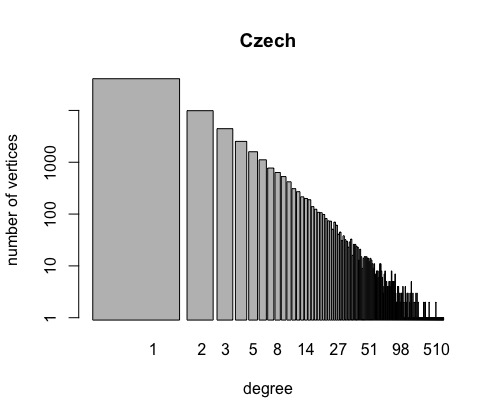
\includegraphics[width=\textwidth]{czech.jpeg}
    \captionsetup{type=figure}
    \captionof{figure}{Czech In Degree}
    \label{fig:czech}
  \end{minipage}

  \begin{minipage}[t]{\linewidth}
    \includegraphics[width=\textwidth]{English}
    \captionsetup{type=figure}
    \captionof{figure}{English In Degree}
    \label{fig:english}
  \end{minipage}

  \begin{minipage}[t]{\linewidth}
    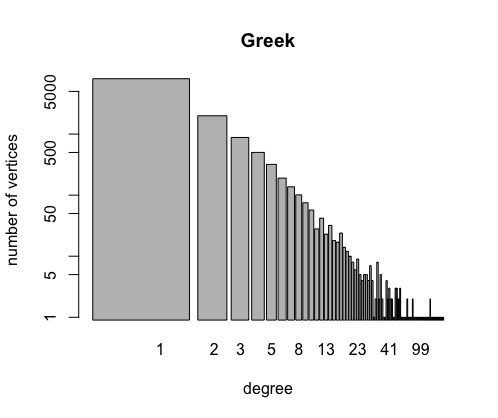
\includegraphics[width=\textwidth]{greek}
    \captionsetup{type=figure}
    \captionof{figure}{Greek In Degree}
    \label{fig:greek}
  \end{minipage}

  \begin{minipage}[t]{\linewidth}
    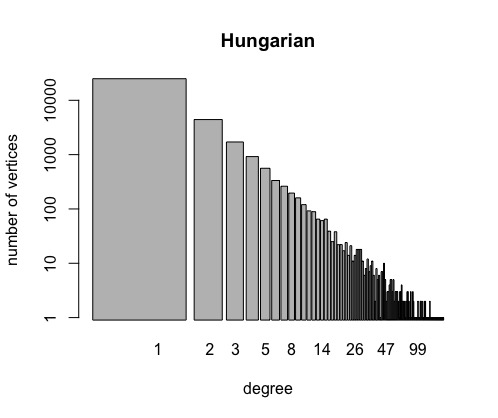
\includegraphics[width=\textwidth]{hungarian}
    \captionsetup{type=figure}
    \captionof{figure}{Hungarian In Degree}
    \label{fig:hungarian}
  \end{minipage}

  \begin{minipage}[t]{\linewidth}
    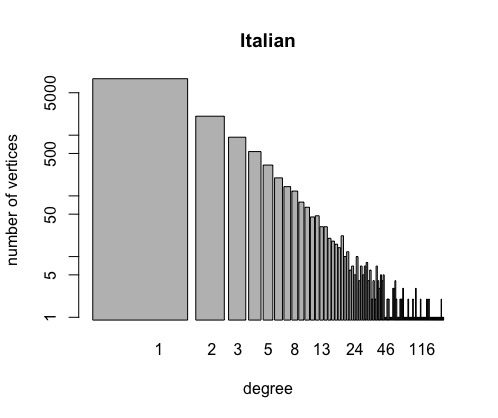
\includegraphics[width=\textwidth]{italian}
    \captionsetup{type=figure}
    \captionof{figure}{Italian In Degree}
    \label{fig:italian}
  \end{minipage}

  \begin{minipage}[t]{\linewidth}
    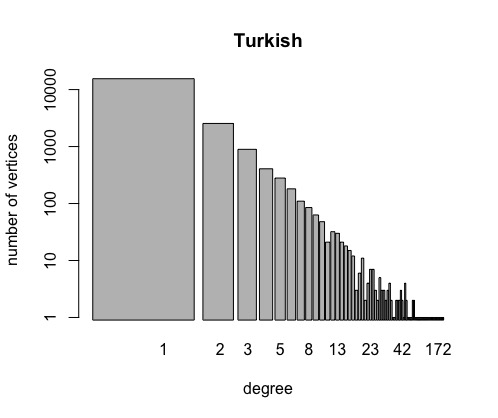
\includegraphics[width=\textwidth]{turkish}
    \captionsetup{type=figure}
    \captionof{figure}{Turkish In Degree}
    \label{fig:turksh}
  \end{minipage}


\section{Source code}
In the source code there are 3 folders with code:


\end{document}